
% Default to the notebook output style

    


% Inherit from the specified cell style.




    
\documentclass[11pt]{article}

    
    
    \usepackage[T1]{fontenc}
    % Nicer default font (+ math font) than Computer Modern for most use cases
    \usepackage{mathpazo}

    % Basic figure setup, for now with no caption control since it's done
    % automatically by Pandoc (which extracts ![](path) syntax from Markdown).
    \usepackage{graphicx}
    % We will generate all images so they have a width \maxwidth. This means
    % that they will get their normal width if they fit onto the page, but
    % are scaled down if they would overflow the margins.
    \makeatletter
    \def\maxwidth{\ifdim\Gin@nat@width>\linewidth\linewidth
    \else\Gin@nat@width\fi}
    \makeatother
    \let\Oldincludegraphics\includegraphics
    % Set max figure width to be 80% of text width, for now hardcoded.
    \renewcommand{\includegraphics}[1]{\Oldincludegraphics[width=.8\maxwidth]{#1}}
    % Ensure that by default, figures have no caption (until we provide a
    % proper Figure object with a Caption API and a way to capture that
    % in the conversion process - todo).
    \usepackage{caption}
    \DeclareCaptionLabelFormat{nolabel}{}
    \captionsetup{labelformat=nolabel}

    \usepackage{adjustbox} % Used to constrain images to a maximum size 
    \usepackage{xcolor} % Allow colors to be defined
    \usepackage{enumerate} % Needed for markdown enumerations to work
    \usepackage{geometry} % Used to adjust the document margins
    \usepackage{amsmath} % Equations
    \usepackage{amssymb} % Equations
    \usepackage{textcomp} % defines textquotesingle
    % Hack from http://tex.stackexchange.com/a/47451/13684:
    \AtBeginDocument{%
        \def\PYZsq{\textquotesingle}% Upright quotes in Pygmentized code
    }
    \usepackage{upquote} % Upright quotes for verbatim code
    \usepackage{eurosym} % defines \euro
    \usepackage[mathletters]{ucs} % Extended unicode (utf-8) support
    \usepackage[utf8x]{inputenc} % Allow utf-8 characters in the tex document
    \usepackage{fancyvrb} % verbatim replacement that allows latex
    \usepackage{grffile} % extends the file name processing of package graphics 
                         % to support a larger range 
    % The hyperref package gives us a pdf with properly built
    % internal navigation ('pdf bookmarks' for the table of contents,
    % internal cross-reference links, web links for URLs, etc.)
    \usepackage{hyperref}
    \usepackage{longtable} % longtable support required by pandoc >1.10
    \usepackage{booktabs}  % table support for pandoc > 1.12.2
    \usepackage[inline]{enumitem} % IRkernel/repr support (it uses the enumerate* environment)
    \usepackage[normalem]{ulem} % ulem is needed to support strikethroughs (\sout)
                                % normalem makes italics be italics, not underlines
    

    
    
    % Colors for the hyperref package
    \definecolor{urlcolor}{rgb}{0,.145,.698}
    \definecolor{linkcolor}{rgb}{.71,0.21,0.01}
    \definecolor{citecolor}{rgb}{.12,.54,.11}

    % ANSI colors
    \definecolor{ansi-black}{HTML}{3E424D}
    \definecolor{ansi-black-intense}{HTML}{282C36}
    \definecolor{ansi-red}{HTML}{E75C58}
    \definecolor{ansi-red-intense}{HTML}{B22B31}
    \definecolor{ansi-green}{HTML}{00A250}
    \definecolor{ansi-green-intense}{HTML}{007427}
    \definecolor{ansi-yellow}{HTML}{DDB62B}
    \definecolor{ansi-yellow-intense}{HTML}{B27D12}
    \definecolor{ansi-blue}{HTML}{208FFB}
    \definecolor{ansi-blue-intense}{HTML}{0065CA}
    \definecolor{ansi-magenta}{HTML}{D160C4}
    \definecolor{ansi-magenta-intense}{HTML}{A03196}
    \definecolor{ansi-cyan}{HTML}{60C6C8}
    \definecolor{ansi-cyan-intense}{HTML}{258F8F}
    \definecolor{ansi-white}{HTML}{C5C1B4}
    \definecolor{ansi-white-intense}{HTML}{A1A6B2}

    % commands and environments needed by pandoc snippets
    % extracted from the output of `pandoc -s`
    \providecommand{\tightlist}{%
      \setlength{\itemsep}{0pt}\setlength{\parskip}{0pt}}
    \DefineVerbatimEnvironment{Highlighting}{Verbatim}{commandchars=\\\{\}}
    % Add ',fontsize=\small' for more characters per line
    \newenvironment{Shaded}{}{}
    \newcommand{\KeywordTok}[1]{\textcolor[rgb]{0.00,0.44,0.13}{\textbf{{#1}}}}
    \newcommand{\DataTypeTok}[1]{\textcolor[rgb]{0.56,0.13,0.00}{{#1}}}
    \newcommand{\DecValTok}[1]{\textcolor[rgb]{0.25,0.63,0.44}{{#1}}}
    \newcommand{\BaseNTok}[1]{\textcolor[rgb]{0.25,0.63,0.44}{{#1}}}
    \newcommand{\FloatTok}[1]{\textcolor[rgb]{0.25,0.63,0.44}{{#1}}}
    \newcommand{\CharTok}[1]{\textcolor[rgb]{0.25,0.44,0.63}{{#1}}}
    \newcommand{\StringTok}[1]{\textcolor[rgb]{0.25,0.44,0.63}{{#1}}}
    \newcommand{\CommentTok}[1]{\textcolor[rgb]{0.38,0.63,0.69}{\textit{{#1}}}}
    \newcommand{\OtherTok}[1]{\textcolor[rgb]{0.00,0.44,0.13}{{#1}}}
    \newcommand{\AlertTok}[1]{\textcolor[rgb]{1.00,0.00,0.00}{\textbf{{#1}}}}
    \newcommand{\FunctionTok}[1]{\textcolor[rgb]{0.02,0.16,0.49}{{#1}}}
    \newcommand{\RegionMarkerTok}[1]{{#1}}
    \newcommand{\ErrorTok}[1]{\textcolor[rgb]{1.00,0.00,0.00}{\textbf{{#1}}}}
    \newcommand{\NormalTok}[1]{{#1}}
    
    % Additional commands for more recent versions of Pandoc
    \newcommand{\ConstantTok}[1]{\textcolor[rgb]{0.53,0.00,0.00}{{#1}}}
    \newcommand{\SpecialCharTok}[1]{\textcolor[rgb]{0.25,0.44,0.63}{{#1}}}
    \newcommand{\VerbatimStringTok}[1]{\textcolor[rgb]{0.25,0.44,0.63}{{#1}}}
    \newcommand{\SpecialStringTok}[1]{\textcolor[rgb]{0.73,0.40,0.53}{{#1}}}
    \newcommand{\ImportTok}[1]{{#1}}
    \newcommand{\DocumentationTok}[1]{\textcolor[rgb]{0.73,0.13,0.13}{\textit{{#1}}}}
    \newcommand{\AnnotationTok}[1]{\textcolor[rgb]{0.38,0.63,0.69}{\textbf{\textit{{#1}}}}}
    \newcommand{\CommentVarTok}[1]{\textcolor[rgb]{0.38,0.63,0.69}{\textbf{\textit{{#1}}}}}
    \newcommand{\VariableTok}[1]{\textcolor[rgb]{0.10,0.09,0.49}{{#1}}}
    \newcommand{\ControlFlowTok}[1]{\textcolor[rgb]{0.00,0.44,0.13}{\textbf{{#1}}}}
    \newcommand{\OperatorTok}[1]{\textcolor[rgb]{0.40,0.40,0.40}{{#1}}}
    \newcommand{\BuiltInTok}[1]{{#1}}
    \newcommand{\ExtensionTok}[1]{{#1}}
    \newcommand{\PreprocessorTok}[1]{\textcolor[rgb]{0.74,0.48,0.00}{{#1}}}
    \newcommand{\AttributeTok}[1]{\textcolor[rgb]{0.49,0.56,0.16}{{#1}}}
    \newcommand{\InformationTok}[1]{\textcolor[rgb]{0.38,0.63,0.69}{\textbf{\textit{{#1}}}}}
    \newcommand{\WarningTok}[1]{\textcolor[rgb]{0.38,0.63,0.69}{\textbf{\textit{{#1}}}}}
    
    
    % Define a nice break command that doesn't care if a line doesn't already
    % exist.
    \def\br{\hspace*{\fill} \\* }
    % Math Jax compatability definitions
    \def\gt{>}
    \def\lt{<}
    % Document parameters
    \title{5.5 Model Selection and Hyperparameter Tuning}
    
    
    

    % Pygments definitions
    
\makeatletter
\def\PY@reset{\let\PY@it=\relax \let\PY@bf=\relax%
    \let\PY@ul=\relax \let\PY@tc=\relax%
    \let\PY@bc=\relax \let\PY@ff=\relax}
\def\PY@tok#1{\csname PY@tok@#1\endcsname}
\def\PY@toks#1+{\ifx\relax#1\empty\else%
    \PY@tok{#1}\expandafter\PY@toks\fi}
\def\PY@do#1{\PY@bc{\PY@tc{\PY@ul{%
    \PY@it{\PY@bf{\PY@ff{#1}}}}}}}
\def\PY#1#2{\PY@reset\PY@toks#1+\relax+\PY@do{#2}}

\expandafter\def\csname PY@tok@w\endcsname{\def\PY@tc##1{\textcolor[rgb]{0.73,0.73,0.73}{##1}}}
\expandafter\def\csname PY@tok@c\endcsname{\let\PY@it=\textit\def\PY@tc##1{\textcolor[rgb]{0.25,0.50,0.50}{##1}}}
\expandafter\def\csname PY@tok@cp\endcsname{\def\PY@tc##1{\textcolor[rgb]{0.74,0.48,0.00}{##1}}}
\expandafter\def\csname PY@tok@k\endcsname{\let\PY@bf=\textbf\def\PY@tc##1{\textcolor[rgb]{0.00,0.50,0.00}{##1}}}
\expandafter\def\csname PY@tok@kp\endcsname{\def\PY@tc##1{\textcolor[rgb]{0.00,0.50,0.00}{##1}}}
\expandafter\def\csname PY@tok@kt\endcsname{\def\PY@tc##1{\textcolor[rgb]{0.69,0.00,0.25}{##1}}}
\expandafter\def\csname PY@tok@o\endcsname{\def\PY@tc##1{\textcolor[rgb]{0.40,0.40,0.40}{##1}}}
\expandafter\def\csname PY@tok@ow\endcsname{\let\PY@bf=\textbf\def\PY@tc##1{\textcolor[rgb]{0.67,0.13,1.00}{##1}}}
\expandafter\def\csname PY@tok@nb\endcsname{\def\PY@tc##1{\textcolor[rgb]{0.00,0.50,0.00}{##1}}}
\expandafter\def\csname PY@tok@nf\endcsname{\def\PY@tc##1{\textcolor[rgb]{0.00,0.00,1.00}{##1}}}
\expandafter\def\csname PY@tok@nc\endcsname{\let\PY@bf=\textbf\def\PY@tc##1{\textcolor[rgb]{0.00,0.00,1.00}{##1}}}
\expandafter\def\csname PY@tok@nn\endcsname{\let\PY@bf=\textbf\def\PY@tc##1{\textcolor[rgb]{0.00,0.00,1.00}{##1}}}
\expandafter\def\csname PY@tok@ne\endcsname{\let\PY@bf=\textbf\def\PY@tc##1{\textcolor[rgb]{0.82,0.25,0.23}{##1}}}
\expandafter\def\csname PY@tok@nv\endcsname{\def\PY@tc##1{\textcolor[rgb]{0.10,0.09,0.49}{##1}}}
\expandafter\def\csname PY@tok@no\endcsname{\def\PY@tc##1{\textcolor[rgb]{0.53,0.00,0.00}{##1}}}
\expandafter\def\csname PY@tok@nl\endcsname{\def\PY@tc##1{\textcolor[rgb]{0.63,0.63,0.00}{##1}}}
\expandafter\def\csname PY@tok@ni\endcsname{\let\PY@bf=\textbf\def\PY@tc##1{\textcolor[rgb]{0.60,0.60,0.60}{##1}}}
\expandafter\def\csname PY@tok@na\endcsname{\def\PY@tc##1{\textcolor[rgb]{0.49,0.56,0.16}{##1}}}
\expandafter\def\csname PY@tok@nt\endcsname{\let\PY@bf=\textbf\def\PY@tc##1{\textcolor[rgb]{0.00,0.50,0.00}{##1}}}
\expandafter\def\csname PY@tok@nd\endcsname{\def\PY@tc##1{\textcolor[rgb]{0.67,0.13,1.00}{##1}}}
\expandafter\def\csname PY@tok@s\endcsname{\def\PY@tc##1{\textcolor[rgb]{0.73,0.13,0.13}{##1}}}
\expandafter\def\csname PY@tok@sd\endcsname{\let\PY@it=\textit\def\PY@tc##1{\textcolor[rgb]{0.73,0.13,0.13}{##1}}}
\expandafter\def\csname PY@tok@si\endcsname{\let\PY@bf=\textbf\def\PY@tc##1{\textcolor[rgb]{0.73,0.40,0.53}{##1}}}
\expandafter\def\csname PY@tok@se\endcsname{\let\PY@bf=\textbf\def\PY@tc##1{\textcolor[rgb]{0.73,0.40,0.13}{##1}}}
\expandafter\def\csname PY@tok@sr\endcsname{\def\PY@tc##1{\textcolor[rgb]{0.73,0.40,0.53}{##1}}}
\expandafter\def\csname PY@tok@ss\endcsname{\def\PY@tc##1{\textcolor[rgb]{0.10,0.09,0.49}{##1}}}
\expandafter\def\csname PY@tok@sx\endcsname{\def\PY@tc##1{\textcolor[rgb]{0.00,0.50,0.00}{##1}}}
\expandafter\def\csname PY@tok@m\endcsname{\def\PY@tc##1{\textcolor[rgb]{0.40,0.40,0.40}{##1}}}
\expandafter\def\csname PY@tok@gh\endcsname{\let\PY@bf=\textbf\def\PY@tc##1{\textcolor[rgb]{0.00,0.00,0.50}{##1}}}
\expandafter\def\csname PY@tok@gu\endcsname{\let\PY@bf=\textbf\def\PY@tc##1{\textcolor[rgb]{0.50,0.00,0.50}{##1}}}
\expandafter\def\csname PY@tok@gd\endcsname{\def\PY@tc##1{\textcolor[rgb]{0.63,0.00,0.00}{##1}}}
\expandafter\def\csname PY@tok@gi\endcsname{\def\PY@tc##1{\textcolor[rgb]{0.00,0.63,0.00}{##1}}}
\expandafter\def\csname PY@tok@gr\endcsname{\def\PY@tc##1{\textcolor[rgb]{1.00,0.00,0.00}{##1}}}
\expandafter\def\csname PY@tok@ge\endcsname{\let\PY@it=\textit}
\expandafter\def\csname PY@tok@gs\endcsname{\let\PY@bf=\textbf}
\expandafter\def\csname PY@tok@gp\endcsname{\let\PY@bf=\textbf\def\PY@tc##1{\textcolor[rgb]{0.00,0.00,0.50}{##1}}}
\expandafter\def\csname PY@tok@go\endcsname{\def\PY@tc##1{\textcolor[rgb]{0.53,0.53,0.53}{##1}}}
\expandafter\def\csname PY@tok@gt\endcsname{\def\PY@tc##1{\textcolor[rgb]{0.00,0.27,0.87}{##1}}}
\expandafter\def\csname PY@tok@err\endcsname{\def\PY@bc##1{\setlength{\fboxsep}{0pt}\fcolorbox[rgb]{1.00,0.00,0.00}{1,1,1}{\strut ##1}}}
\expandafter\def\csname PY@tok@kc\endcsname{\let\PY@bf=\textbf\def\PY@tc##1{\textcolor[rgb]{0.00,0.50,0.00}{##1}}}
\expandafter\def\csname PY@tok@kd\endcsname{\let\PY@bf=\textbf\def\PY@tc##1{\textcolor[rgb]{0.00,0.50,0.00}{##1}}}
\expandafter\def\csname PY@tok@kn\endcsname{\let\PY@bf=\textbf\def\PY@tc##1{\textcolor[rgb]{0.00,0.50,0.00}{##1}}}
\expandafter\def\csname PY@tok@kr\endcsname{\let\PY@bf=\textbf\def\PY@tc##1{\textcolor[rgb]{0.00,0.50,0.00}{##1}}}
\expandafter\def\csname PY@tok@bp\endcsname{\def\PY@tc##1{\textcolor[rgb]{0.00,0.50,0.00}{##1}}}
\expandafter\def\csname PY@tok@fm\endcsname{\def\PY@tc##1{\textcolor[rgb]{0.00,0.00,1.00}{##1}}}
\expandafter\def\csname PY@tok@vc\endcsname{\def\PY@tc##1{\textcolor[rgb]{0.10,0.09,0.49}{##1}}}
\expandafter\def\csname PY@tok@vg\endcsname{\def\PY@tc##1{\textcolor[rgb]{0.10,0.09,0.49}{##1}}}
\expandafter\def\csname PY@tok@vi\endcsname{\def\PY@tc##1{\textcolor[rgb]{0.10,0.09,0.49}{##1}}}
\expandafter\def\csname PY@tok@vm\endcsname{\def\PY@tc##1{\textcolor[rgb]{0.10,0.09,0.49}{##1}}}
\expandafter\def\csname PY@tok@sa\endcsname{\def\PY@tc##1{\textcolor[rgb]{0.73,0.13,0.13}{##1}}}
\expandafter\def\csname PY@tok@sb\endcsname{\def\PY@tc##1{\textcolor[rgb]{0.73,0.13,0.13}{##1}}}
\expandafter\def\csname PY@tok@sc\endcsname{\def\PY@tc##1{\textcolor[rgb]{0.73,0.13,0.13}{##1}}}
\expandafter\def\csname PY@tok@dl\endcsname{\def\PY@tc##1{\textcolor[rgb]{0.73,0.13,0.13}{##1}}}
\expandafter\def\csname PY@tok@s2\endcsname{\def\PY@tc##1{\textcolor[rgb]{0.73,0.13,0.13}{##1}}}
\expandafter\def\csname PY@tok@sh\endcsname{\def\PY@tc##1{\textcolor[rgb]{0.73,0.13,0.13}{##1}}}
\expandafter\def\csname PY@tok@s1\endcsname{\def\PY@tc##1{\textcolor[rgb]{0.73,0.13,0.13}{##1}}}
\expandafter\def\csname PY@tok@mb\endcsname{\def\PY@tc##1{\textcolor[rgb]{0.40,0.40,0.40}{##1}}}
\expandafter\def\csname PY@tok@mf\endcsname{\def\PY@tc##1{\textcolor[rgb]{0.40,0.40,0.40}{##1}}}
\expandafter\def\csname PY@tok@mh\endcsname{\def\PY@tc##1{\textcolor[rgb]{0.40,0.40,0.40}{##1}}}
\expandafter\def\csname PY@tok@mi\endcsname{\def\PY@tc##1{\textcolor[rgb]{0.40,0.40,0.40}{##1}}}
\expandafter\def\csname PY@tok@il\endcsname{\def\PY@tc##1{\textcolor[rgb]{0.40,0.40,0.40}{##1}}}
\expandafter\def\csname PY@tok@mo\endcsname{\def\PY@tc##1{\textcolor[rgb]{0.40,0.40,0.40}{##1}}}
\expandafter\def\csname PY@tok@ch\endcsname{\let\PY@it=\textit\def\PY@tc##1{\textcolor[rgb]{0.25,0.50,0.50}{##1}}}
\expandafter\def\csname PY@tok@cm\endcsname{\let\PY@it=\textit\def\PY@tc##1{\textcolor[rgb]{0.25,0.50,0.50}{##1}}}
\expandafter\def\csname PY@tok@cpf\endcsname{\let\PY@it=\textit\def\PY@tc##1{\textcolor[rgb]{0.25,0.50,0.50}{##1}}}
\expandafter\def\csname PY@tok@c1\endcsname{\let\PY@it=\textit\def\PY@tc##1{\textcolor[rgb]{0.25,0.50,0.50}{##1}}}
\expandafter\def\csname PY@tok@cs\endcsname{\let\PY@it=\textit\def\PY@tc##1{\textcolor[rgb]{0.25,0.50,0.50}{##1}}}

\def\PYZbs{\char`\\}
\def\PYZus{\char`\_}
\def\PYZob{\char`\{}
\def\PYZcb{\char`\}}
\def\PYZca{\char`\^}
\def\PYZam{\char`\&}
\def\PYZlt{\char`\<}
\def\PYZgt{\char`\>}
\def\PYZsh{\char`\#}
\def\PYZpc{\char`\%}
\def\PYZdl{\char`\$}
\def\PYZhy{\char`\-}
\def\PYZsq{\char`\'}
\def\PYZdq{\char`\"}
\def\PYZti{\char`\~}
% for compatibility with earlier versions
\def\PYZat{@}
\def\PYZlb{[}
\def\PYZrb{]}
\makeatother


    % Exact colors from NB
    \definecolor{incolor}{rgb}{0.0, 0.0, 0.5}
    \definecolor{outcolor}{rgb}{0.545, 0.0, 0.0}



    
    % Prevent overflowing lines due to hard-to-break entities
    \sloppy 
    % Setup hyperref package
    \hypersetup{
      breaklinks=true,  % so long urls are correctly broken across lines
      colorlinks=true,
      urlcolor=urlcolor,
      linkcolor=linkcolor,
      citecolor=citecolor,
      }
    % Slightly bigger margins than the latex defaults
    
    \geometry{verbose,tmargin=1in,bmargin=1in,lmargin=1in,rmargin=1in}
    
    

    \begin{document}
    
    
    \maketitle
    
    

    
    \hypertarget{model-selection-and-hyperparameter-tuning}{%
\section{5.5 Model Selection and Hyperparameter
Tuning}\label{model-selection-and-hyperparameter-tuning}}

This section will use the tools developed in the previous section to
answer two important questions:

\begin{itemize}
\tightlist
\item
  Model Selection: How do we determine which model is best?
\item
  Hyperparameter Tuning: How do we choose hyperparameters, such as \(k\)
  in \(k\)-nearest neighbors?
\end{itemize}

In the previous section, we saw how to use training and validation sets
to estimate how well the model will perform on future data. A natural
way to decide between competing models (or hyperparameters) is to choose
the one that minimizes the validation error.

    \begin{Verbatim}[commandchars=\\\{\}]
{\color{incolor}In [{\color{incolor}4}]:} \PY{o}{\PYZpc{}}\PY{k}{matplotlib} inline
        \PY{k+kn}{import} \PY{n+nn}{numpy} \PY{k}{as} \PY{n+nn}{np}
        \PY{k+kn}{import} \PY{n+nn}{pandas} \PY{k}{as} \PY{n+nn}{pd}
        \PY{n}{pd}\PY{o}{.}\PY{n}{options}\PY{o}{.}\PY{n}{display}\PY{o}{.}\PY{n}{max\PYZus{}rows} \PY{o}{=} \PY{l+m+mi}{5}
        
        \PY{n}{housing} \PY{o}{=} \PY{n}{pd}\PY{o}{.}\PY{n}{read\PYZus{}csv}\PY{p}{(}\PY{l+s+s2}{\PYZdq{}}\PY{l+s+s2}{https://raw.githubusercontent.com/dlsun/data\PYZhy{}science\PYZhy{}book/master/data/AmesHousing.txt}\PY{l+s+s2}{\PYZdq{}}\PY{p}{,}
                              \PY{n}{sep}\PY{o}{=}\PY{l+s+s2}{\PYZdq{}}\PY{l+s+se}{\PYZbs{}t}\PY{l+s+s2}{\PYZdq{}}\PY{p}{)}
        \PY{n}{housing}
\end{Verbatim}


\begin{Verbatim}[commandchars=\\\{\}]
{\color{outcolor}Out[{\color{outcolor}4}]:}       Order        PID  MS SubClass MS Zoning  Lot Frontage  Lot Area Street  \textbackslash{}
        0         1  526301100           20        RL         141.0     31770   Pave   
        1         2  526350040           20        RH          80.0     11622   Pave   
        {\ldots}     {\ldots}        {\ldots}          {\ldots}       {\ldots}           {\ldots}       {\ldots}    {\ldots}   
        2928   2929  924100070           20        RL          77.0     10010   Pave   
        2929   2930  924151050           60        RL          74.0      9627   Pave   
        
             Alley Lot Shape Land Contour    {\ldots}     Pool Area Pool QC  Fence  \textbackslash{}
        0      NaN       IR1          Lvl    {\ldots}             0     NaN    NaN   
        1      NaN       Reg          Lvl    {\ldots}             0     NaN  MnPrv   
        {\ldots}    {\ldots}       {\ldots}          {\ldots}    {\ldots}           {\ldots}     {\ldots}    {\ldots}   
        2928   NaN       Reg          Lvl    {\ldots}             0     NaN    NaN   
        2929   NaN       Reg          Lvl    {\ldots}             0     NaN    NaN   
        
             Misc Feature Misc Val Mo Sold Yr Sold Sale Type  Sale Condition  \textbackslash{}
        0             NaN        0       5    2010       WD           Normal   
        1             NaN        0       6    2010       WD           Normal   
        {\ldots}           {\ldots}      {\ldots}     {\ldots}     {\ldots}       {\ldots}             {\ldots}   
        2928          NaN        0       4    2006       WD           Normal   
        2929          NaN        0      11    2006       WD           Normal   
        
              SalePrice  
        0        215000  
        1        105000  
        {\ldots}         {\ldots}  
        2928     170000  
        2929     188000  
        
        [2930 rows x 82 columns]
\end{Verbatim}
            
    \hypertarget{k-fold-cross-validation}{%
\subsection{\texorpdfstring{\(K\)-Fold Cross
Validation}{K-Fold Cross Validation}}\label{k-fold-cross-validation}}

Previously, we carried out cross validation by splitting the data into 2
halves, alternately using one half to train the model and the other to
evaluate the model. In general, we can split the data into \(k\)
subsamples, alternately training the data on \(k-1\) subsamples and
evaluating the model on the \(1\) remaining subsample, i.e., the
validation set. This produces \(k\) somewhat independent estimates of
the test error. This procedure is known as \textbf{\(k\)-fold cross
validation}. (Be careful not to confuse the \(k\) in \(k\)-fold cross
validation with the \(k\) in \(k\)-nearest neighbors.) Therefore, the
specific version of cross validation that we saw earlier is \(2\)-fold
cross validation.

A schematic of \(4\)-fold cross validation is shown below.

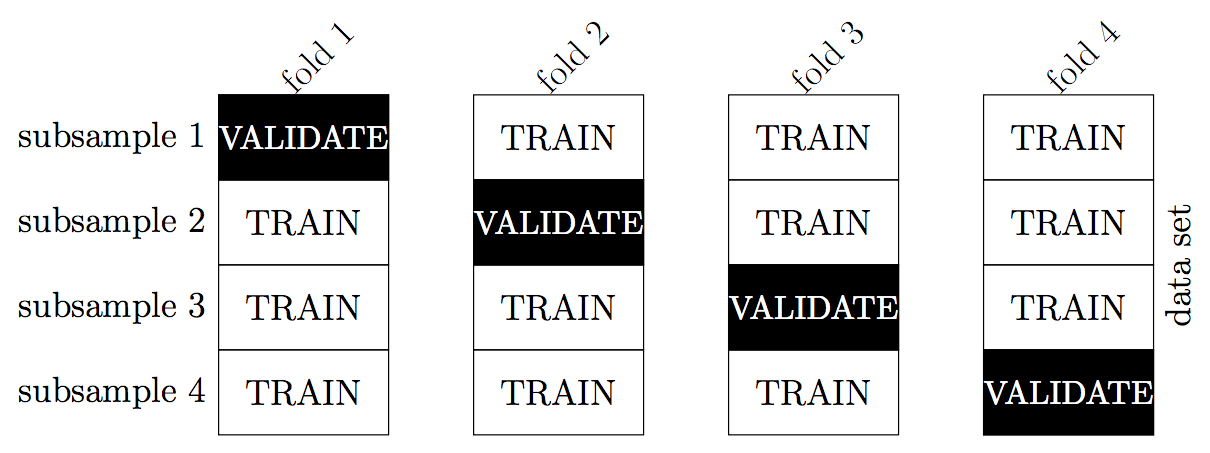
\includegraphics{k-folds.png}

Implementing \(k\)-fold cross validation from scratch for \(k > 2\) is
straightforward but messy, so we will usually let Scikit-Learn do it for
us.

    \hypertarget{cross-validation-in-scikit-learn}{%
\subsection{Cross Validation in
Scikit-Learn}\label{cross-validation-in-scikit-learn}}

Scikit-Learn provides a function, \texttt{cross\_val\_score}, that will
carry out all aspects of \(k\)-fold cross validation:

\begin{enumerate}
\def\labelenumi{\arabic{enumi}.}
\tightlist
\item
  split the data into \(k\) subsamples
\item
  combine the first \(k-1\) subsamples into a training set and train the
  model
\item
  evaluate the model predictions on the last (\(k\)th) held-out
  subsample
\item
  repeat steps 2-3 \(k\) times (i.e.~\(k\) ``folds''), each time holding
  out a different one of the \(k\) subsamples
\item
  calculate \(k\) ``scores'', one from each validation set
\end{enumerate}

There is one subtlety to keep in mind. Training a \(k\)-nearest
neighbors model is not just about fitting the model; it also involves
dummifying the categorical variables and scaling the variables. These
preprocessing steps should be included in the cross-validation process.
They cannot be done ahead of time.

For example, suppose we run \(5\)-fold cross validation. Then:

\begin{itemize}
\tightlist
\item
  When subsamples 1-4 are used for training and subsample 5 for
  validation, the observations have to be standardized with respect to
  the mean and SD of subsamples 1-4.
\item
  When subsamples 2-5 are used for training and subsample 1 for
  validation, the observations have to be standardized with respect to
  the mean and SD of subsamples 2-5.
\item
  And so on.
\end{itemize}

We cannot simply standardize all of the data once at the beginning and
run cross validation on the standardized data. To do so would be
allowing the model to peek at the validation set during training. That's
because each training set would be standardized with respect to a mean
and SD that is calculated from all data, including the validation set.
To be completely above board, we should standardize each training set
with respect to the mean and SD of just that training set.

Fortunately, Scikit-Learn provides a \texttt{Pipeline} object that
allows us to chain these preprocessing steps together with the model we
want to fit.

    \begin{Verbatim}[commandchars=\\\{\}]
{\color{incolor}In [{\color{incolor}5}]:} \PY{k+kn}{from} \PY{n+nn}{sklearn}\PY{n+nn}{.}\PY{n+nn}{feature\PYZus{}extraction} \PY{k}{import} \PY{n}{DictVectorizer}
        \PY{k+kn}{from} \PY{n+nn}{sklearn}\PY{n+nn}{.}\PY{n+nn}{preprocessing} \PY{k}{import} \PY{n}{StandardScaler}
        \PY{k+kn}{from} \PY{n+nn}{sklearn}\PY{n+nn}{.}\PY{n+nn}{neighbors} \PY{k}{import} \PY{n}{KNeighborsRegressor}
        \PY{k+kn}{from} \PY{n+nn}{sklearn}\PY{n+nn}{.}\PY{n+nn}{pipeline} \PY{k}{import} \PY{n}{Pipeline}
        
        \PY{c+c1}{\PYZsh{} get the features (in dict format) and the labels}
        \PY{c+c1}{\PYZsh{} (do not split into training and validation sets)}
        \PY{n}{features} \PY{o}{=} \PY{p}{[}\PY{l+s+s2}{\PYZdq{}}\PY{l+s+s2}{Lot Area}\PY{l+s+s2}{\PYZdq{}}\PY{p}{,} \PY{l+s+s2}{\PYZdq{}}\PY{l+s+s2}{Gr Liv Area}\PY{l+s+s2}{\PYZdq{}}\PY{p}{,}
                    \PY{l+s+s2}{\PYZdq{}}\PY{l+s+s2}{Full Bath}\PY{l+s+s2}{\PYZdq{}}\PY{p}{,} \PY{l+s+s2}{\PYZdq{}}\PY{l+s+s2}{Half Bath}\PY{l+s+s2}{\PYZdq{}}\PY{p}{,}
                    \PY{l+s+s2}{\PYZdq{}}\PY{l+s+s2}{Bedroom AbvGr}\PY{l+s+s2}{\PYZdq{}}\PY{p}{,} 
                    \PY{l+s+s2}{\PYZdq{}}\PY{l+s+s2}{Year Built}\PY{l+s+s2}{\PYZdq{}}\PY{p}{,} \PY{l+s+s2}{\PYZdq{}}\PY{l+s+s2}{Yr Sold}\PY{l+s+s2}{\PYZdq{}}\PY{p}{,}
                    \PY{l+s+s2}{\PYZdq{}}\PY{l+s+s2}{Neighborhood}\PY{l+s+s2}{\PYZdq{}}\PY{p}{]}
        \PY{n}{X\PYZus{}dict} \PY{o}{=} \PY{n}{housing}\PY{p}{[}\PY{n}{features}\PY{p}{]}\PY{o}{.}\PY{n}{to\PYZus{}dict}\PY{p}{(}\PY{n}{orient}\PY{o}{=}\PY{l+s+s2}{\PYZdq{}}\PY{l+s+s2}{records}\PY{l+s+s2}{\PYZdq{}}\PY{p}{)}
        \PY{n}{y} \PY{o}{=} \PY{n}{housing}\PY{p}{[}\PY{l+s+s2}{\PYZdq{}}\PY{l+s+s2}{SalePrice}\PY{l+s+s2}{\PYZdq{}}\PY{p}{]}
        
        \PY{c+c1}{\PYZsh{} specify the pipeline}
        \PY{n}{vec} \PY{o}{=} \PY{n}{DictVectorizer}\PY{p}{(}\PY{n}{sparse}\PY{o}{=}\PY{k+kc}{False}\PY{p}{)}
        \PY{n}{scaler} \PY{o}{=} \PY{n}{StandardScaler}\PY{p}{(}\PY{p}{)}
        \PY{n}{model} \PY{o}{=} \PY{n}{KNeighborsRegressor}\PY{p}{(}\PY{n}{n\PYZus{}neighbors}\PY{o}{=}\PY{l+m+mi}{10}\PY{p}{)}
        \PY{n}{pipeline} \PY{o}{=} \PY{n}{Pipeline}\PY{p}{(}\PY{p}{[}\PY{p}{(}\PY{l+s+s2}{\PYZdq{}}\PY{l+s+s2}{vectorizer}\PY{l+s+s2}{\PYZdq{}}\PY{p}{,} \PY{n}{vec}\PY{p}{)}\PY{p}{,} \PY{p}{(}\PY{l+s+s2}{\PYZdq{}}\PY{l+s+s2}{scaler}\PY{l+s+s2}{\PYZdq{}}\PY{p}{,} \PY{n}{scaler}\PY{p}{)}\PY{p}{,} \PY{p}{(}\PY{l+s+s2}{\PYZdq{}}\PY{l+s+s2}{fit}\PY{l+s+s2}{\PYZdq{}}\PY{p}{,} \PY{n}{model}\PY{p}{)}\PY{p}{]}\PY{p}{)}
\end{Verbatim}


    This entire \texttt{Pipeline} can be passed to
\texttt{cross\_val\_score}, along with the data, the number of folds
\(k\) (\texttt{cv}), and the type of score (\texttt{scoring}). So
\(5\)-fold cross validation in Scikit-Learn would look as follows:

    \begin{Verbatim}[commandchars=\\\{\}]
{\color{incolor}In [{\color{incolor}6}]:} \PY{k+kn}{from} \PY{n+nn}{sklearn}\PY{n+nn}{.}\PY{n+nn}{model\PYZus{}selection} \PY{k}{import} \PY{n}{cross\PYZus{}val\PYZus{}score}
        
        \PY{n}{scores} \PY{o}{=} \PY{n}{cross\PYZus{}val\PYZus{}score}\PY{p}{(}\PY{n}{pipeline}\PY{p}{,} \PY{n}{X\PYZus{}dict}\PY{p}{,} \PY{n}{y}\PY{p}{,} 
                                 \PY{n}{cv}\PY{o}{=}\PY{l+m+mi}{5}\PY{p}{,} \PY{n}{scoring}\PY{o}{=}\PY{l+s+s2}{\PYZdq{}}\PY{l+s+s2}{neg\PYZus{}mean\PYZus{}squared\PYZus{}error}\PY{l+s+s2}{\PYZdq{}}\PY{p}{)}
        \PY{n}{scores}
\end{Verbatim}


\begin{Verbatim}[commandchars=\\\{\}]
{\color{outcolor}Out[{\color{outcolor}6}]:} array([ -1.98025092e+09,  -1.47950953e+09,  -1.54632969e+09,
                -1.87662563e+09,  -1.42167566e+09])
\end{Verbatim}
            
    Notice that we get five (negative) validation MSEs, one from each of the
5 folds. \texttt{cross\_val\_score} returns the \emph{negative} MSE,
instead of the MSE, because by definition, a \emph{higher} score is
better. (Since we want the MSE to be as \emph{low} as possible, we want
the negative MSE to be as \emph{high} as possible.)

To come up with a single overall estimate of the test MSE, we flip the
signs and average the MSEs:

    \begin{Verbatim}[commandchars=\\\{\}]
{\color{incolor}In [{\color{incolor}7}]:} \PY{n}{np}\PY{o}{.}\PY{n}{mean}\PY{p}{(}\PY{o}{\PYZhy{}}\PY{n}{scores}\PY{p}{)}
\end{Verbatim}


\begin{Verbatim}[commandchars=\\\{\}]
{\color{outcolor}Out[{\color{outcolor}7}]:} 1660878287.4356349
\end{Verbatim}
            
    The RMSE is the square root of the MSE:

    \begin{Verbatim}[commandchars=\\\{\}]
{\color{incolor}In [{\color{incolor}8}]:} \PY{n}{np}\PY{o}{.}\PY{n}{sqrt}\PY{p}{(}\PY{n}{np}\PY{o}{.}\PY{n}{mean}\PY{p}{(}\PY{o}{\PYZhy{}}\PY{n}{scores}\PY{p}{)}\PY{p}{)}
\end{Verbatim}


\begin{Verbatim}[commandchars=\\\{\}]
{\color{outcolor}Out[{\color{outcolor}8}]:} 40753.874508267734
\end{Verbatim}
            
    \hypertarget{hyperparameter-tuning}{%
\subsection{Hyperparameter Tuning}\label{hyperparameter-tuning}}

How do we choose \(k\)? We can simply try all values of \(k\) and pick
the one with the smallest (test) MSE.

    \begin{Verbatim}[commandchars=\\\{\}]
{\color{incolor}In [{\color{incolor}9}]:} \PY{n}{vec} \PY{o}{=} \PY{n}{DictVectorizer}\PY{p}{(}\PY{n}{sparse}\PY{o}{=}\PY{k+kc}{False}\PY{p}{)}
        \PY{n}{scaler} \PY{o}{=} \PY{n}{StandardScaler}\PY{p}{(}\PY{p}{)}
        
        \PY{c+c1}{\PYZsh{} calculates estimate of test error based on 10\PYZhy{}fold cross validation}
        \PY{k}{def} \PY{n+nf}{get\PYZus{}cv\PYZus{}error}\PY{p}{(}\PY{n}{k}\PY{p}{)}\PY{p}{:}
            \PY{n}{model} \PY{o}{=} \PY{n}{KNeighborsRegressor}\PY{p}{(}\PY{n}{n\PYZus{}neighbors}\PY{o}{=}\PY{n}{k}\PY{p}{)}
            \PY{n}{pipeline} \PY{o}{=} \PY{n}{Pipeline}\PY{p}{(}\PY{p}{[}\PY{p}{(}\PY{l+s+s2}{\PYZdq{}}\PY{l+s+s2}{vectorizer}\PY{l+s+s2}{\PYZdq{}}\PY{p}{,} \PY{n}{vec}\PY{p}{)}\PY{p}{,} \PY{p}{(}\PY{l+s+s2}{\PYZdq{}}\PY{l+s+s2}{scaler}\PY{l+s+s2}{\PYZdq{}}\PY{p}{,} \PY{n}{scaler}\PY{p}{)}\PY{p}{,} \PY{p}{(}\PY{l+s+s2}{\PYZdq{}}\PY{l+s+s2}{fit}\PY{l+s+s2}{\PYZdq{}}\PY{p}{,} \PY{n}{model}\PY{p}{)}\PY{p}{]}\PY{p}{)}
            \PY{n}{mse} \PY{o}{=} \PY{n}{np}\PY{o}{.}\PY{n}{mean}\PY{p}{(}\PY{o}{\PYZhy{}}\PY{n}{cross\PYZus{}val\PYZus{}score}\PY{p}{(}
                \PY{n}{pipeline}\PY{p}{,} \PY{n}{X\PYZus{}dict}\PY{p}{,} \PY{n}{y}\PY{p}{,} 
                \PY{n}{cv}\PY{o}{=}\PY{l+m+mi}{10}\PY{p}{,} \PY{n}{scoring}\PY{o}{=}\PY{l+s+s2}{\PYZdq{}}\PY{l+s+s2}{neg\PYZus{}mean\PYZus{}squared\PYZus{}error}\PY{l+s+s2}{\PYZdq{}}
            \PY{p}{)}\PY{p}{)}
            \PY{k}{return} \PY{n}{mse}
            
        \PY{n}{ks} \PY{o}{=} \PY{n}{pd}\PY{o}{.}\PY{n}{Series}\PY{p}{(}\PY{n+nb}{range}\PY{p}{(}\PY{l+m+mi}{1}\PY{p}{,} \PY{l+m+mi}{51}\PY{p}{)}\PY{p}{)}
        \PY{n}{ks}\PY{o}{.}\PY{n}{index} \PY{o}{=} \PY{n+nb}{range}\PY{p}{(}\PY{l+m+mi}{1}\PY{p}{,} \PY{l+m+mi}{51}\PY{p}{)}
        \PY{n}{test\PYZus{}errs} \PY{o}{=} \PY{n}{ks}\PY{o}{.}\PY{n}{apply}\PY{p}{(}\PY{n}{get\PYZus{}cv\PYZus{}error}\PY{p}{)}
        
        \PY{n}{test\PYZus{}errs}\PY{o}{.}\PY{n}{plot}\PY{o}{.}\PY{n}{line}\PY{p}{(}\PY{p}{)}
        \PY{n}{test\PYZus{}errs}\PY{o}{.}\PY{n}{sort\PYZus{}values}\PY{p}{(}\PY{p}{)}
\end{Verbatim}


\begin{Verbatim}[commandchars=\\\{\}]
{\color{outcolor}Out[{\color{outcolor}9}]:} 4     1.390511e+09
        3     1.405909e+09
                  {\ldots}     
        49    2.208727e+09
        50    2.216495e+09
        Length: 50, dtype: float64
\end{Verbatim}
            
    \begin{center}
    \adjustimage{max size={0.9\linewidth}{0.9\paperheight}}{output_12_1.png}
    \end{center}
    { \hspace*{\fill} \\}
    
    The MSE is minimized near \(k = 4\), which suggests that a \(4\)-nearest
neighbors model is optimal for prediction.

    \hypertarget{model-selection}{%
\subsection{Model Selection}\label{model-selection}}

Suppose we are not sure whether \texttt{Yr\ Sold} should be included in
the \(4\)-nearest neighbors model or not. To determine whether or not it
should be included, we can fit a model with \texttt{Yr\ Sold} included
and another model with it excluded, and see which model has the better
(test) MSE.

    \begin{Verbatim}[commandchars=\\\{\}]
{\color{incolor}In [{\color{incolor}10}]:} \PY{n}{vec} \PY{o}{=} \PY{n}{DictVectorizer}\PY{p}{(}\PY{n}{sparse}\PY{o}{=}\PY{k+kc}{False}\PY{p}{)}
         \PY{n}{scaler} \PY{o}{=} \PY{n}{StandardScaler}\PY{p}{(}\PY{p}{)}
         \PY{n}{model} \PY{o}{=} \PY{n}{KNeighborsRegressor}\PY{p}{(}\PY{n}{n\PYZus{}neighbors}\PY{o}{=}\PY{l+m+mi}{4}\PY{p}{)}
         \PY{n}{pipeline} \PY{o}{=} \PY{n}{Pipeline}\PY{p}{(}\PY{p}{[}\PY{p}{(}\PY{l+s+s2}{\PYZdq{}}\PY{l+s+s2}{vectorizer}\PY{l+s+s2}{\PYZdq{}}\PY{p}{,} \PY{n}{vec}\PY{p}{)}\PY{p}{,} \PY{p}{(}\PY{l+s+s2}{\PYZdq{}}\PY{l+s+s2}{scaler}\PY{l+s+s2}{\PYZdq{}}\PY{p}{,} \PY{n}{scaler}\PY{p}{)}\PY{p}{,} \PY{p}{(}\PY{l+s+s2}{\PYZdq{}}\PY{l+s+s2}{fit}\PY{l+s+s2}{\PYZdq{}}\PY{p}{,} \PY{n}{model}\PY{p}{)}\PY{p}{]}\PY{p}{)}
\end{Verbatim}


    \begin{Verbatim}[commandchars=\\\{\}]
{\color{incolor}In [{\color{incolor}11}]:} \PY{n}{features} \PY{o}{=} \PY{p}{[}\PY{l+s+s2}{\PYZdq{}}\PY{l+s+s2}{Lot Area}\PY{l+s+s2}{\PYZdq{}}\PY{p}{,} \PY{l+s+s2}{\PYZdq{}}\PY{l+s+s2}{Gr Liv Area}\PY{l+s+s2}{\PYZdq{}}\PY{p}{,}
                     \PY{l+s+s2}{\PYZdq{}}\PY{l+s+s2}{Full Bath}\PY{l+s+s2}{\PYZdq{}}\PY{p}{,} \PY{l+s+s2}{\PYZdq{}}\PY{l+s+s2}{Half Bath}\PY{l+s+s2}{\PYZdq{}}\PY{p}{,}
                     \PY{l+s+s2}{\PYZdq{}}\PY{l+s+s2}{Bedroom AbvGr}\PY{l+s+s2}{\PYZdq{}}\PY{p}{,} 
                     \PY{l+s+s2}{\PYZdq{}}\PY{l+s+s2}{Year Built}\PY{l+s+s2}{\PYZdq{}}\PY{p}{,} \PY{l+s+s2}{\PYZdq{}}\PY{l+s+s2}{Yr Sold}\PY{l+s+s2}{\PYZdq{}}\PY{p}{,}
                     \PY{l+s+s2}{\PYZdq{}}\PY{l+s+s2}{Neighborhood}\PY{l+s+s2}{\PYZdq{}}\PY{p}{]}
         \PY{n}{X\PYZus{}dict} \PY{o}{=} \PY{n}{housing}\PY{p}{[}\PY{n}{features}\PY{p}{]}\PY{o}{.}\PY{n}{to\PYZus{}dict}\PY{p}{(}\PY{n}{orient}\PY{o}{=}\PY{l+s+s2}{\PYZdq{}}\PY{l+s+s2}{records}\PY{l+s+s2}{\PYZdq{}}\PY{p}{)}
         \PY{n}{np}\PY{o}{.}\PY{n}{mean}\PY{p}{(}
             \PY{o}{\PYZhy{}}\PY{n}{cross\PYZus{}val\PYZus{}score}\PY{p}{(}\PY{n}{pipeline}\PY{p}{,} \PY{n}{X\PYZus{}dict}\PY{p}{,} \PY{n}{y}\PY{p}{,} \PY{n}{cv}\PY{o}{=}\PY{l+m+mi}{10}\PY{p}{,} \PY{n}{scoring}\PY{o}{=}\PY{l+s+s2}{\PYZdq{}}\PY{l+s+s2}{neg\PYZus{}mean\PYZus{}squared\PYZus{}error}\PY{l+s+s2}{\PYZdq{}}\PY{p}{)}
         \PY{p}{)}
\end{Verbatim}


\begin{Verbatim}[commandchars=\\\{\}]
{\color{outcolor}Out[{\color{outcolor}11}]:} 1390511354.3758318
\end{Verbatim}
            
    \begin{Verbatim}[commandchars=\\\{\}]
{\color{incolor}In [{\color{incolor}12}]:} \PY{n}{features} \PY{o}{=} \PY{p}{[}\PY{l+s+s2}{\PYZdq{}}\PY{l+s+s2}{Lot Area}\PY{l+s+s2}{\PYZdq{}}\PY{p}{,} \PY{l+s+s2}{\PYZdq{}}\PY{l+s+s2}{Gr Liv Area}\PY{l+s+s2}{\PYZdq{}}\PY{p}{,}
                     \PY{l+s+s2}{\PYZdq{}}\PY{l+s+s2}{Full Bath}\PY{l+s+s2}{\PYZdq{}}\PY{p}{,} \PY{l+s+s2}{\PYZdq{}}\PY{l+s+s2}{Half Bath}\PY{l+s+s2}{\PYZdq{}}\PY{p}{,}
                     \PY{l+s+s2}{\PYZdq{}}\PY{l+s+s2}{Bedroom AbvGr}\PY{l+s+s2}{\PYZdq{}}\PY{p}{,} 
                     \PY{l+s+s2}{\PYZdq{}}\PY{l+s+s2}{Year Built}\PY{l+s+s2}{\PYZdq{}}\PY{p}{,}
                     \PY{l+s+s2}{\PYZdq{}}\PY{l+s+s2}{Neighborhood}\PY{l+s+s2}{\PYZdq{}}\PY{p}{]}
         \PY{n}{X\PYZus{}dict} \PY{o}{=} \PY{n}{housing}\PY{p}{[}\PY{n}{features}\PY{p}{]}\PY{o}{.}\PY{n}{to\PYZus{}dict}\PY{p}{(}\PY{n}{orient}\PY{o}{=}\PY{l+s+s2}{\PYZdq{}}\PY{l+s+s2}{records}\PY{l+s+s2}{\PYZdq{}}\PY{p}{)}
         \PY{o}{\PYZhy{}}\PY{n}{cross\PYZus{}val\PYZus{}score}\PY{p}{(}\PY{n}{pipeline}\PY{p}{,} \PY{n}{X\PYZus{}dict}\PY{p}{,} \PY{n}{y}\PY{p}{,} \PY{n}{cv}\PY{o}{=}\PY{l+m+mi}{10}\PY{p}{,} \PY{n}{scoring}\PY{o}{=}\PY{l+s+s2}{\PYZdq{}}\PY{l+s+s2}{neg\PYZus{}mean\PYZus{}squared\PYZus{}error}\PY{l+s+s2}{\PYZdq{}}\PY{p}{)}\PY{o}{.}\PY{n}{mean}\PY{p}{(}\PY{p}{)}
\end{Verbatim}


\begin{Verbatim}[commandchars=\\\{\}]
{\color{outcolor}Out[{\color{outcolor}12}]:} 1315348887.0818686
\end{Verbatim}
            
    The MSE actually goes down when we remove \texttt{Yr\ Sold}, so it seems
that the model is better off without this variable.


    % Add a bibliography block to the postdoc
    
    
    
    \end{document}
